\documentclass[
germanthesis
]{i3thesis}
% options:
% [germanthesis] - Thesis is written in German
% [plainunnumbered] - Don't print numbers on plain pages
% [earlydraft] - Settings for quick draft printouts
% [watermark] - Print current time/date at bottom of each page
% [phdthesis] - switch to PhD thesis style
% [twoside] - double sided

\usepackage{multirow}
\usepackage{floatflt}
%\usepackage[babel=true]{csquotes}
%\usepackage[backend=biber,style=ieee]{biblatex}

%% CUSTOM
% ------------------------------

% for figures
\usepackage{caption}
\usepackage{subcaption}
\usepackage{tocloft}

% subchapters in capital
\newcommand{\sh}[1]{%
  \vspace{1em}%
  \noindent\MakeUppercase{#1}\\%
}

% acronyms
\iffalse
\newcommand{\listofacronyms}{%
  \chapter*{\glossarytitlename}%
  \addcontentsline{toc}{chapter}{\glossarytitlename}%
  \begin{acronym}[XXXX] % Longest acronym for alignment
    % The acronyms will be listed here
  \end{acronym}%
}

\renewcommand{\acronymname}{\glossarytitlename}
\renewcommand{\acronymfont}[1]{\textbf{#1}}
\setlength{\acronymindent}{0em}
\setlength{\acronymlabelwidth}{4em}
\setlength{\acronymlabelsep}{1em}
\fi

% tables
\usepackage{csvsimple}
\usepackage{booktabs}
\usepackage{longtable}
\usepackage{pdflscape}
\usepackage{adjustbox} % in preamble

 % ------------------------------

\author{Dustin Heither}
\title{Best Practices und Trends bei didaktischen Simulatoren für Rechnerarchitektur:
Eine systematische Literaturrecherche}
\thesistype{Bachelorarbeit}
\thesiscite{Bachelor's Thesis~(Bachelorarbeit)}
\birthday{10. Mai 1992}
\birthplace{Oberhausen}
\thesisstart{30. April 2025}
\advisors{M.Sc. Tobias Baumeister}

\addbibresource{thesis.bib}
\graphicspath{{images/},{pictures/}}

\begin{document}
\pagenumbering{roman}

\maketitle
\acresetall

\cleardoublepage
\tableofcontents

\iffalse
\cleardoublepage
\listofacronyms
\begin{acronym}[1234567890]
\end{acronym}

\fi

\cleardoublepage
\pagenumbering{arabic}

\chapter{Einleitung}

\section{Motivation}

Die nachfolgende Bachelorarbeit behandelt das Thema "Best Practices und Trends bei didaktischen Simulatoren für Rechnerarchitektur: Eine systematische Literaturrecherche". Sie wurde am Lehrstuhl für Rechnerarchitektur der Universität Erlangen-Nürnberg im Sommersemester 2025 geschrieben und bildet die abschließende Prüfungsleistung des Bachelorstudiums Informatik.



\section{Zielsetzung}

Innerhalb dieser Arbeit werden Simulatoren vorgestellt und untersucht, die Relevanz in den Themengebieten der Rechnerarchitektur haben und für didaktische Zwecke genutzt werden.

\section{Aufbau der Arbeit}

\chapter{Methodik}

\section{Recherche und Auswahl der Simulatoren}

\section{Kriterienkatalog}

Tabelle~\ref{tab:kriterien} fasst die für die Analyse herangezogenen Kriterien zusammen.

Ein zentrales Kriterium ist der \textit{Zugriff}. Je nach organisatorischem Kontext ist entscheidend, ob ein Simulator online oder offline verfügbar ist. Während eine Online-Lösung eine Internetverbindung erfordert und dadurch eingeschränkt nutzbar sein kann, setzt ein Offline-Simulator häufig eine Installation voraus, die wiederum von Betriebssystem oder Hardwareanforderungen abhängt.

Die \textit{Programmiersprache} ist insbesondere für Studierende der Informatik von Relevanz. Sie kann die Möglichkeit eröffnen, Erweiterungen oder Plugins zu entwickeln und den Simulator an spezifische Bedürfnisse anzupassen.

Unter dem Kriterium \textit{Simulatorart} wird der Abstraktionsgrad eingeordnet, also ob der Simulator didaktisch reduziert oder realitätsnah ist. Ergänzend werden auch die Visualisierung und der Grad der Interaktivität berücksichtigt.

Das Kriterium \textit{Zielgruppe} erlaubt eine Zuordnung zu unterschiedlichen Bildungskontexten (z. B. Schule, Hochschule) und gibt Auskunft darüber, ob und in welchem Umfang Vorkenntnisse erforderlich sind.

Für Lehrende spielt zudem der \textit{Preis} eine zentrale Rolle. Es wird unterschieden, ob es sich um freie oder lizenzpflichtige Software handelt, da der Kostenfaktor maßgeblich über den praktischen Einsatz entscheidet.

Ein weiterer Aspekt ist die \textit{Gamification}. Studien zeigen, dass spielerische Elemente die Lernmotivation steigern können. Unterschieden werden hier insbesondere levelbasierte und storytelling-orientierte Ansätze.\TODO{Referenz einfügen}

Da die Rechnerarchitektur eine Vielzahl von \textit{Themenbereichen} abdeckt, wird erfasst, auf welchen inhaltlichen Schwerpunkt sich ein Simulator bezieht (z. B. Pipelining oder Caching).

Unter \textit{Beschäftigungsdauer} wird die zu erwartende Nutzungszeit betrachtet. Dabei ist relevant, ob die Dauer der Auseinandersetzung mit dem Simulator die notwendige Einführungs- und Erklärungszeit übersteigt.

Die Qualität der \textit{Dokumentation} ist ein weiteres zentrales Kriterium. Eine klare und umfassende Dokumentation erleichtert Installation, Anwendung und Problemlösung und wirkt sich direkt auf die Nutzbarkeit des Simulators aus.

Da die Arbeit auch Trends und Entwicklungen berücksichtigt, werden zudem der \textit{Bekanntheitsgrad}, der \textit{Wartungsstand} (letztes Update) sowie das Jahr der \textit{Veröffentlichung} aufgenommen, um den Stellenwert eines Simulators einzuordnen und veraltete Software zu identifizieren.

\begin{table}[h!]

\centering
\caption{Kriterienkatalog}
\label{tab:kriterien}
\small

\begin{tabular}{|l|l|l|}
\hline

\textbf{Nr.} & \textbf{Kriterien} & \textbf{Kategorie} \\
\hline

\multirow{4}{*}{1} & \multirow{4}{*}{Zugriff} & Offline \\
                   &                          & Betriebssystem \\
                   &                          & Online \\
                   &                          & Hardwareanforderungen \\
\hline

\multirow{3}{*}{2} & \multirow{3}{*}{Programmiersprache} & Entwicklungssprache \\
                   &                                     & Embedding von Programmiersprachen \\
                   &                                     & Integration in Lernplattformen \\
\hline

\multirow{3}{*}{3} & \multirow{3}{*}{Simulatorart} & Abstraktionsgrad \\
                   &                               & Visualisierung \\
                   &                               & Interaktivität \\
\hline

\multirow{2}{*}{4} & \multirow{2}{*}{Zielgruppe} & Institution \\
                   &                             & Vorkenntnisse \\
\hline

\multirow{2}{*}{5} & \multirow{2}{*}{Preis} & Freeware \\
                   &                        & Open Source \\
\hline

\multirow{2}{*}{6} & \multirow{2}{*}{Gamification} & Level \\
                   &                               & Storytelling \\
\hline

\multirow{2}{*}{7} & \multirow{2}{*}{Themenbereich} & Pipelining \\ 
                   &                                & Caching \\
\hline

\multirow{3}{*}{8} & \multirow{3}{*}{Beschäftigungsdauer} & kurzfrisitg \\
                   &                                      & mittelfristig \\
                   &                                      & langfrisitig \\ 
\hline

\multirow{2}{*}{9} & \multirow{2}{*}{Dokumentation} & Verfügbarkeit \\
                   &                                & Zugriff \\
\hline

10 & Bekanntheitsgrad & Skala von 0 - 10 \\
\hline

11 & Wartungsstand & letztes Update \\
\hline

12 & Veröffentlichung & Aktualität \\
\hline

\end{tabular}
\end{table}

\section{Limitierungen}

\chapter{Theoretische Grundlagen}

\section{Didaktische Simulatoren in der Lehre - Relevanz und Herausforderungen}

\section{Konzepte und Lernziele}


"Law of Effect" (deutsch: \textit{Gesetz der Wirkung oder Effektgesetz}) des amerikanischen Psychologen Edward L. Thorndike. Sie zählt zu den Grundlagen wissenschaftlicher Lerntheorien, insbesondere im Bereich des Behaviorismus und der operanten Konditionierung.

Einordnung Simulator als E-Learning?

Gamification

M-Learning

Was ist ein Simulator

Blended Learning

\begin{itemize}
    \item Gamification
    \item Gamified Learning
    \item 4 Modi vom Lernen: Aktiv, Passiv, konstruktiv, interaktiv
\end{itemize}

\section{Definition und Arten von Simulatoren}

\chapter{Ergebnisse der Literatur- und Simulatorrecherche}\label{chap:4-results}

\section{Ergebnisse aus Tabelle~\ref{tab:literatur}}

Das folgende Kapitel fasst die Ergebnisse der systematischen Literaturanalyse zusammen (vgl. Tabelle~\ref{tab:literatur}). Dabei werden die in Kapitel~\ref{chap:kriterienkatalog} definierten Kriterien auf die identifizierten Publikationen angewendet.

\vspace{1em}

Insgesamt umfasst die Analyse 151 Veröffentlichungen, die in Tabelle~\ref{tab:literatur} aufgeführt sind. Abbildung~\ref{fig:1-veroeffentlichungen-jahr} zeigt die jährliche Verteilung der Publikationen. Von den insgesamt 151 Arbeiten wurden 58 im Zeitraum von 2020 bis 2025 veröffentlicht, was einem Anteil von ca. 38~\% entspricht, während weitere 55~\% der Publikationen in den Jahren 2000 bis 2020 erschienen.

\begin{figure}[!htbp]
    \centering
    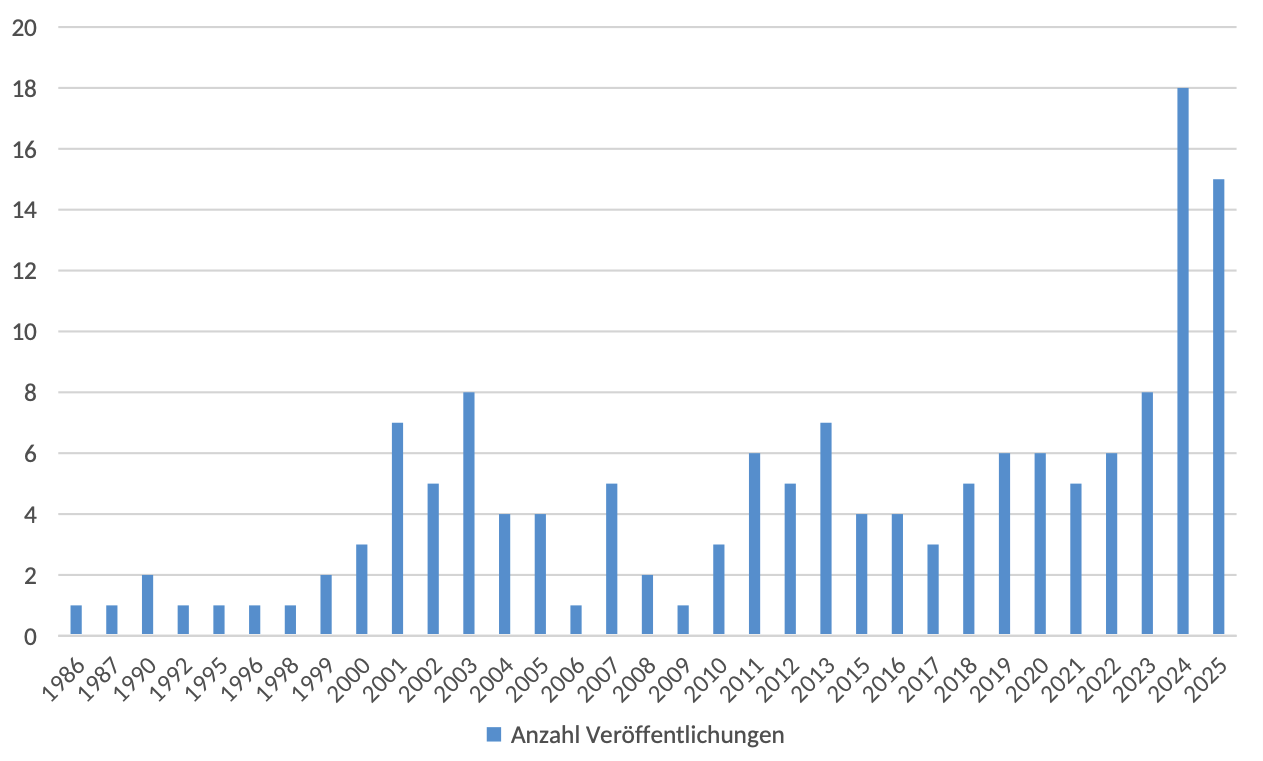
\includegraphics[width=0.90\textwidth]{graphics_lit/1-veroeffentlichungen-jahr.png}
    \caption{Übersicht der Veröffentlichungen pro Jahr}
    \label{fig:1-veroeffentlichungen-jahr}
\end{figure}

Aus Abbildung~\ref{fig:2-typ} ist ersichtlich, dass insgesamt 98~\% der Veröffentlichungen auf Journalartikel (ca. 36~\%) und Konferenzbeiträge (ca. 62~\%) entfallen. Während Journalartikel in Fachzeitschriften mit ausführlicherem Begutachtungsprozess erscheinen, werden Konferenzbeiträge überwiegend in Tagungsbänden veröffentlicht und dienen der schnellen Verbreitung aktueller Forschungsergebnisse \cite{abbadia_conference_2022}. Beide Publikationstypen sind daher für eine Trendanalyse sowie zur Ableitung von Best Practices geeignet.

\begin{figure}[!htbp]
    \centering
    % --- linke Seite: Grafik ---
    \begin{subfigure}[b]{0.48\textwidth}
        \centering
        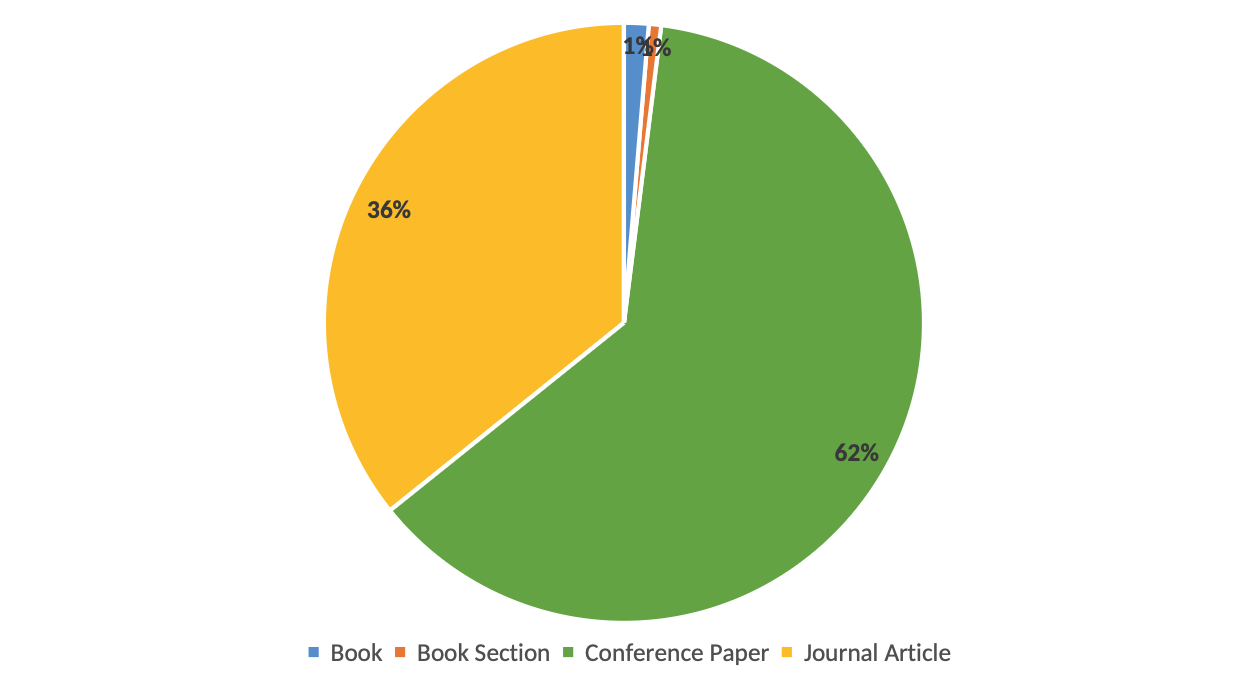
\includegraphics[width=1\textwidth]{graphics_lit/2-typ.png}
        \caption{Übersicht des Typs} 
        \label{fig:2-typ}
    \end{subfigure}
    \hfill
    % 
    % --- rechte Seite: Tabelle ---
    \begin{subfigure}[b]{0.48\textwidth}
        \centering
        \tiny
        \begin{tabularx}{\textwidth}{X c}
            \hline
            \multicolumn{2}{l}{\textbf{Journals}} \\
            \hline
            IEEE Transactions on Education & 10 \\
            Computer Applications in Engineering Education & 7 \\
            Journal on Educational Resources in Computing & 7 \\
            \hline
            \multicolumn{2}{l}{\textbf{Konferenzen}} \\
            \hline
            Workshop on Computer Architecture Education & 8 \\
            ACM Technical Symposium on Computer Science Education & 7 \\
            Annual International Symposium on Computer Architecture & 6 \\
            \hline
        \end{tabularx}
        \caption{Meistgenutzte Journals und Konferenzen}
        \label{tab:2-typ-detail}
    \end{subfigure}
    %
    \caption{Informationen zum Typ der Publikationen}
    \label{fig:2-typ-gesamt}
\end{figure}

Tabelle~\ref{tab:2-typ-detail} bietet eine Übersicht über die Zeitschriften und Konferenzen, in denen die meisten der untersuchten Publikationen veröffentlicht wurden. Die drei genannten Zeitschriften vereinen 44~\% aller Journalartikel, während die drei aufgeführten Konferenzen rund 22~\% der Konferenzbeiträge ausmachen.

Abbildung~\ref{fig:3-anzahl-themen} verdeutlicht, dass die häufigsten Themen der untersuchten Publikationen \enquote{Prozessoren und Architekturen} (44~\%), \enquote{Speicher und Performance} (11~\%) sowie \enquote{Hardware und Logistik} (10~\%) sind. Diese drei Themen umfassen zusammen rund 70~\% aller Publikationen. Dicht darauf folgen die Themen \enquote{Grundlagen und Theorien} sowie \enquote{Programmierung} mit jeweils 9~\% der Arbeiten.

\begin{figure}[!h]
    \centering
    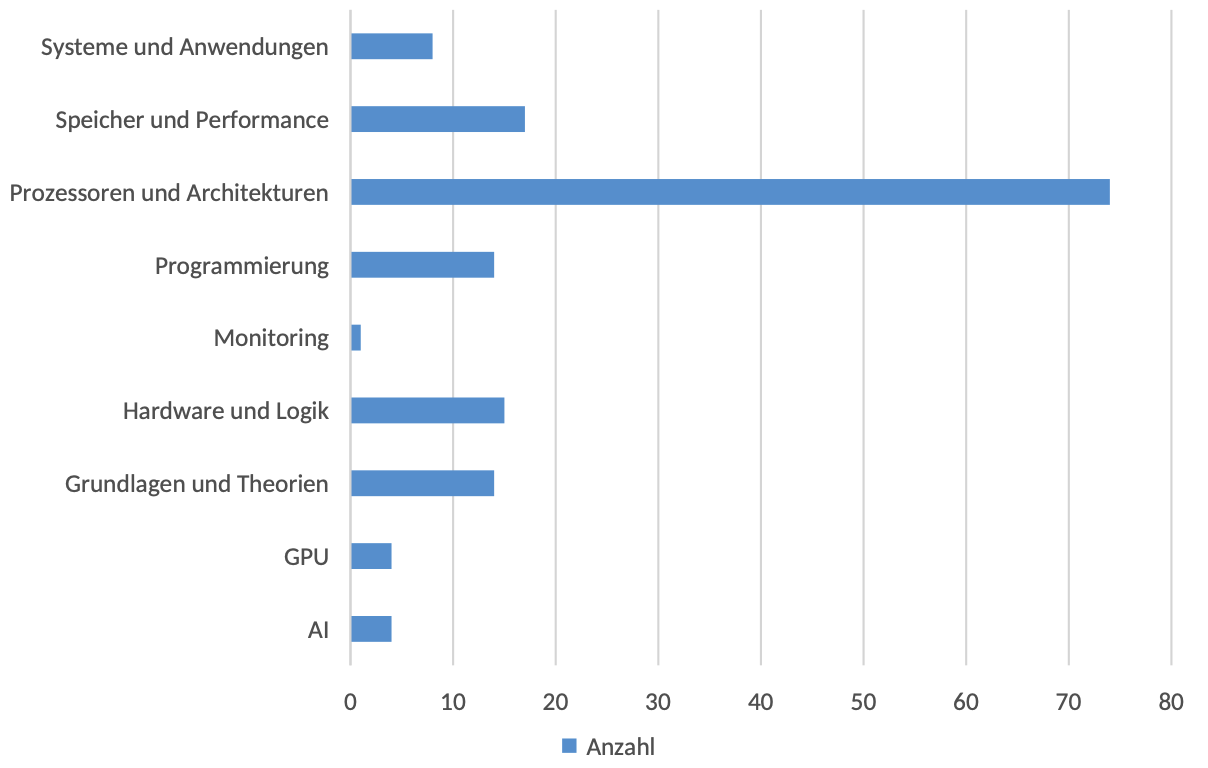
\includegraphics[width=0.90\textwidth]{graphics_lit/3-thema.png}
    \caption{Anzahl der Veröffentlichungen pro Thema}
    \label{fig:3-anzahl-themen}
\end{figure}

Eine detaillierte Untersuchung der drei am häufigsten vertretenen Themen ist in Abbildung~\ref{fig:4-top3-themen} dargestellt. Diese Grafik zeigt die Verteilung dieser Themen über verschiedene Zeitspannen. Die zugrunde liegenden Werte sind in der Tabelle~\ref{tab:themen-zeit} aufgeführt.

\begin{figure}[!htbp]
    \centering
    % --- linke Seite: Grafik ---
    \begin{subfigure}[b]{0.48\textwidth}
        \centering
        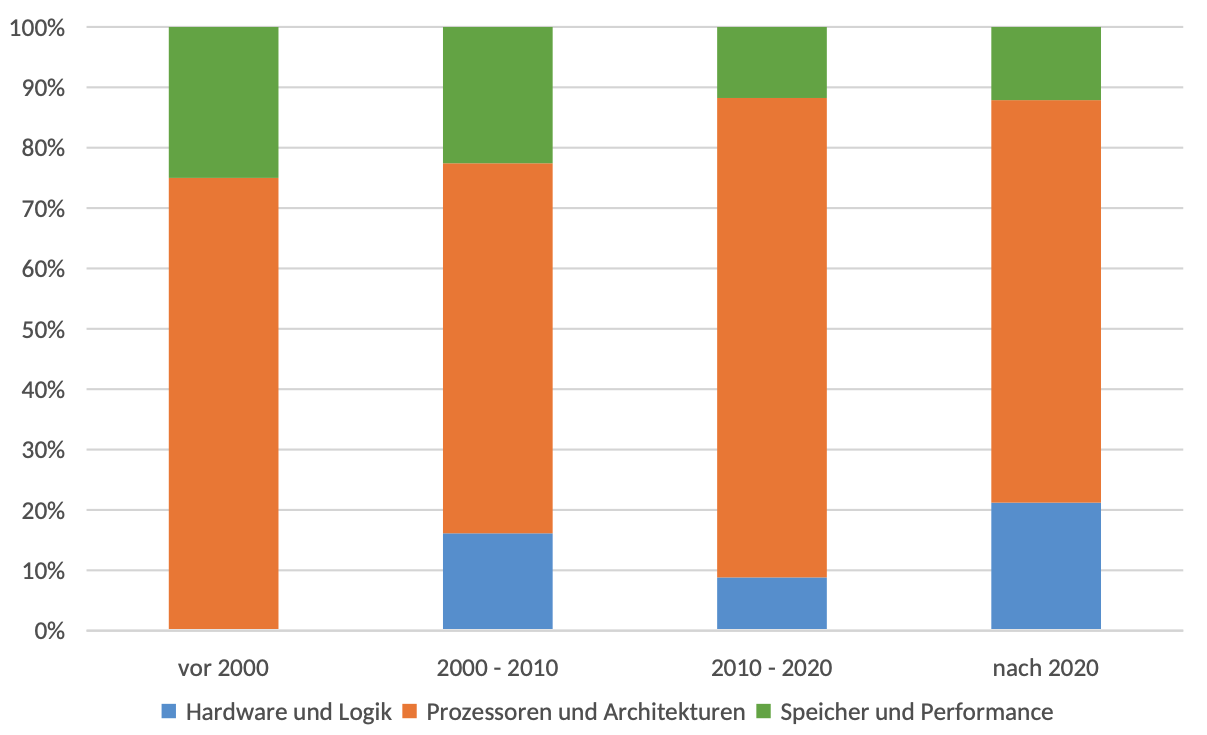
\includegraphics[width=0.90\textwidth]{graphics_lit/4-top3-themen-jahr.png}
        \caption{Jährliche Aufteilung Top 3 Themen (grafisch)}
        \label{fig:4-top3-themen}
    \end{subfigure}
    \hfill
    % 
    % --- rechte Seite: Tabelle ---
    \begin{subfigure}[b]{0.48\textwidth}
        \centering
        \tiny
        \begin{tabularx}{\textwidth}{lXXX}
            \hline
            \textbf{Zeitraum} & \textbf{Hardware und Logik} & \textbf{Prozessoren und Architekturen} & \textbf{Speicher und Performance} \\
            \hline
            vor 2000      & 0  & 6  & 2 \\
            2000--2010    & 5  & 19 & 7 \\
            2010--2020    & 3  & 27 & 4 \\
            nach 2020     & 7  & 22 & 4 \\
            \hline
        \end{tabularx}
        \caption{Jährliche Aufteilung Top 3 Themen (detailliert)}
        \label{tab:themen-zeit}
    \end{subfigure}
    %
    \caption{Jährliche Aufteilung Top 3 Themen}
    \label{fig:pub-typen}
\end{figure}

Für die Themen \enquote{Grundlagen und Theorien} sowie \enquote{Programmierung} zeigt Abb.~\ref{fig:5-top5-themen} die jährliche Verteilung. Die entsprechenden Werte sind in Tab.~\ref{tab:themen-zeit-2} aufgeführt. Auf eine detaillierte Analyse der verbleibenden Themen wir hier verzichtet. In dem Kapitel~\ref{chap:5-discussion} werde die Entwicklung aller Themen aufgegriffen und analysiert.

\begin{figure}[!htbp]
    \centering
    % --- linke Seite: Grafik ---
    \begin{subfigure}[b]{0.48\textwidth}
        \centering
        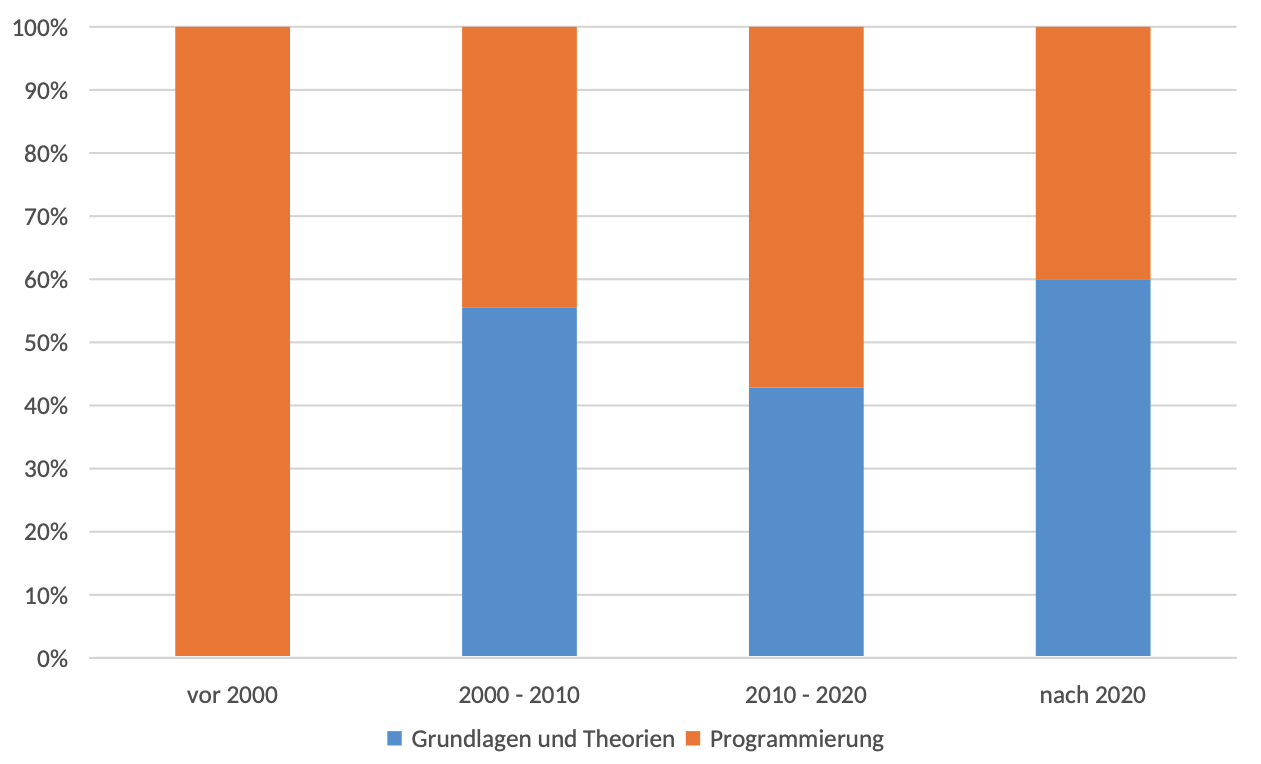
\includegraphics[width=0.90\textwidth]{graphics_lit/5-top5-themen-jahr.png}
        \caption{Jährliche Aufteilung weitere Themen (grafisch)}
        \label{fig:5-top5-themen}
    \end{subfigure}
    \hfill
    % 
    % --- rechte Seite: Tabelle ---
    \begin{subfigure}[b]{0.48\textwidth}
        \centering
        \tiny
        \begin{tabularx}{\textwidth}{lXX}
            \hline
            \textbf{Zeitraum} & \textbf{Grundlagen und Theorien} & \textbf{Programmierung} \\
            \hline
            vor 2000      & 0 & 2 \\
            2000--2010    & 5 & 4 \\
            2010--2020    & 3 & 4 \\
            nach 2020     & 6 & 4 \\
            \hline
        \end{tabularx}
        \caption{Jährliche Aufteilung weitere Themen (detailliert)}
        \label{tab:themen-zeit-2}
    \end{subfigure}
    %
    \caption{Jährliche Aufteilung weitere Themen}
    \label{fig:pub-typen}
\end{figure}

Hinsichtlich der Frage, ob die untersuchten Simulatoren spielerische Elemente (\textit{Gamification}) enthalten, bietet die Tabelle~\ref{tab:gamification} einen Überblick.

\begin{table}[!htbp]
    \centering
    \tiny
    \begin{tabular}{l c c}
        \hline
        \textbf{Gamification} & \textbf{Anzahl} & \textbf{\%} \\
        \hline
        Keine Elemente     & 145 & 96\% \\
        Elemente vorhanden & 6   & 4\%  \\
        \hline
        \textbf{Summe}     & 151 & 100\% \\
        \hline
    \end{tabular}
    \caption{Verteilung der Publikationen in Bezug auf enthaltene Gamification-Elemente}
    \label{tab:gamification}
\end{table}

Von den 151 Simulatoren der untersuchten wissenschaftlichen Publikationen wurden 15~\% als realitätsnah und 85~\% als didaktisch reduziert eingestuft. Die Verteilung bezogen auf die einzelnen Themenbereiche ist in Abbildung~\ref{fig:7-abstraktion-themen} dargestellt.

Die Abbildung~\ref{fig:8-abstraktion-jahr} verdeutlicht die zeitliche Entwicklung des Abstraktionslevels.

\begin{figure}[!htbp]
    \centering
    % --- linke Seite: Grafik ---
    \begin{subfigure}[b]{0.48\textwidth}
        \centering
        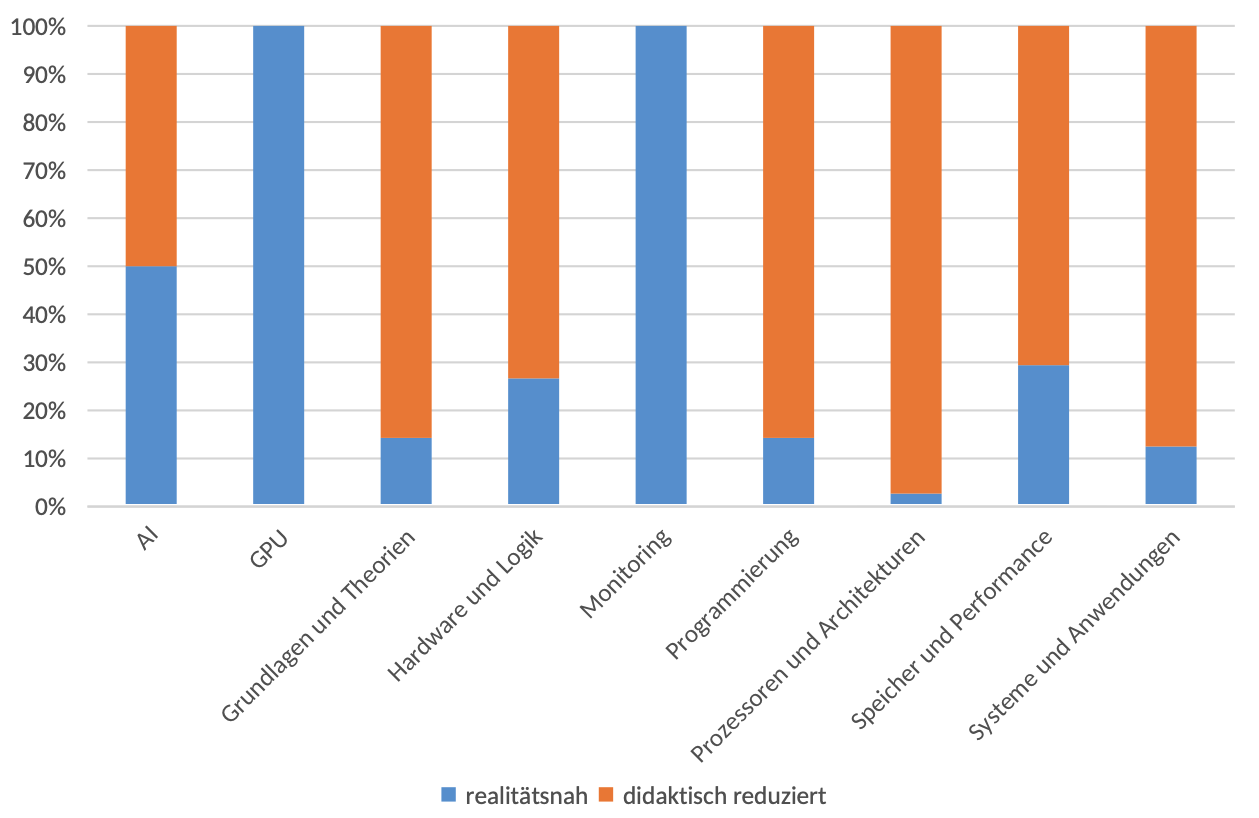
\includegraphics[width=0.90\textwidth]{graphics_lit/7-abtraktion-themen.png}
        \caption{Verteilung Abstraktionslevel auf Themen}
        \label{fig:7-abstraktion-themen}
    \end{subfigure}
    \hfill
    % 
    % --- rechte Seite: Grafik ---
    \begin{subfigure}[b]{0.48\textwidth}
        \centering
        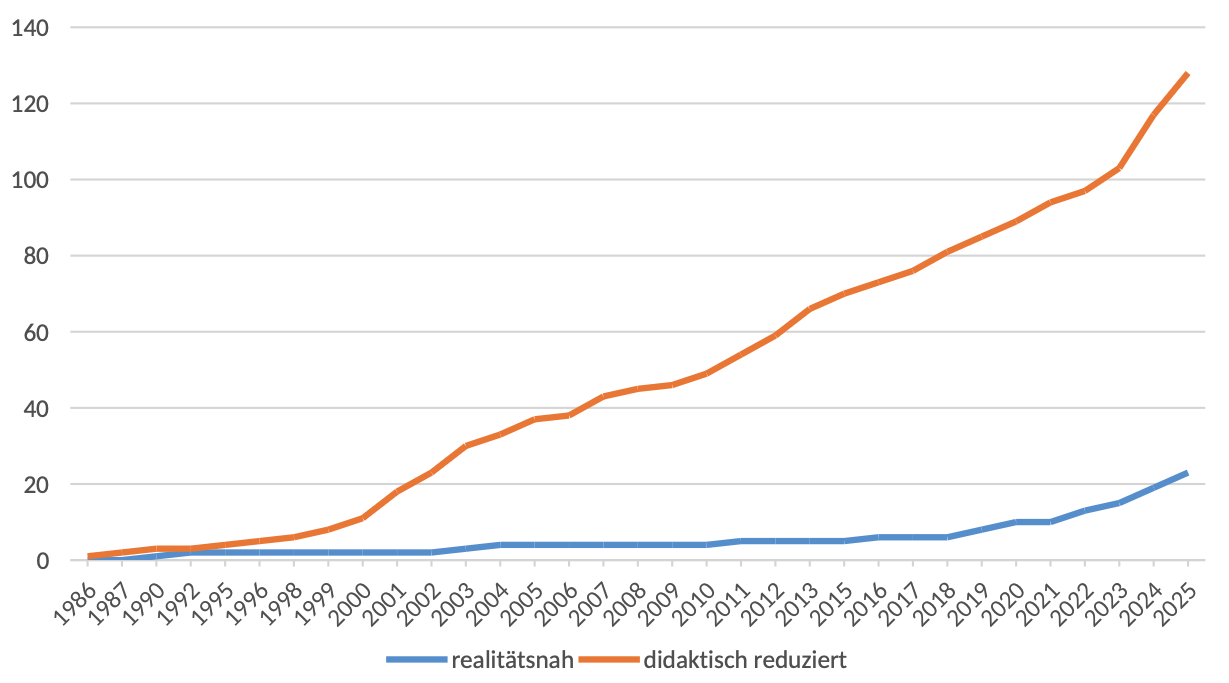
\includegraphics[width=0.90\textwidth]{graphics_lit/8-abstraktion-jahr.png}
        \caption{Zeitliche Entwicklung des Abstraktionslevels}
        \label{fig:8-abstraktion-jahr}
    \end{subfigure}
    %
    \caption{Analysen zum Abstraktionslevel}
    \label{fig:abstaktion-analysen}
\end{figure}

Anhand von Abbildung~\ref{fig:9-institution} ist zu erkennen, dass 89~\% der Publikationen die Hochschulbildung als Zielgruppe adressieren. 9~\% der untersuchten Simulatoren sind für Forschung und Beruf bestimmt, während sich die verbleibenden 2~\% auf schulische Bildung und Weiterbildungen aufteilen.

Untersucht man die Verteilung der Zielgruppen genauer, so zeigt Abbildung~\ref{fig:10-institution-themen} die Aufteilung der einzelnen Zielgruppen (\enquote{Schule}, \enquote{Hochschule}, \enquote{Forschung/Beruf}, \enquote{Weiterbildung}) auf die jeweiligen Themenbereiche. Dabei wird zum Beispiel deutlich, dass sich alle GPU-bezogenen Simulatoren der Forschungs- bzw. Berufsgruppe zuordnen lassen.

\begin{figure}[!htbp]
    \centering
    % --- linke Seite: Grafik ---
    \begin{subfigure}[b]{0.48\textwidth}
        \centering
        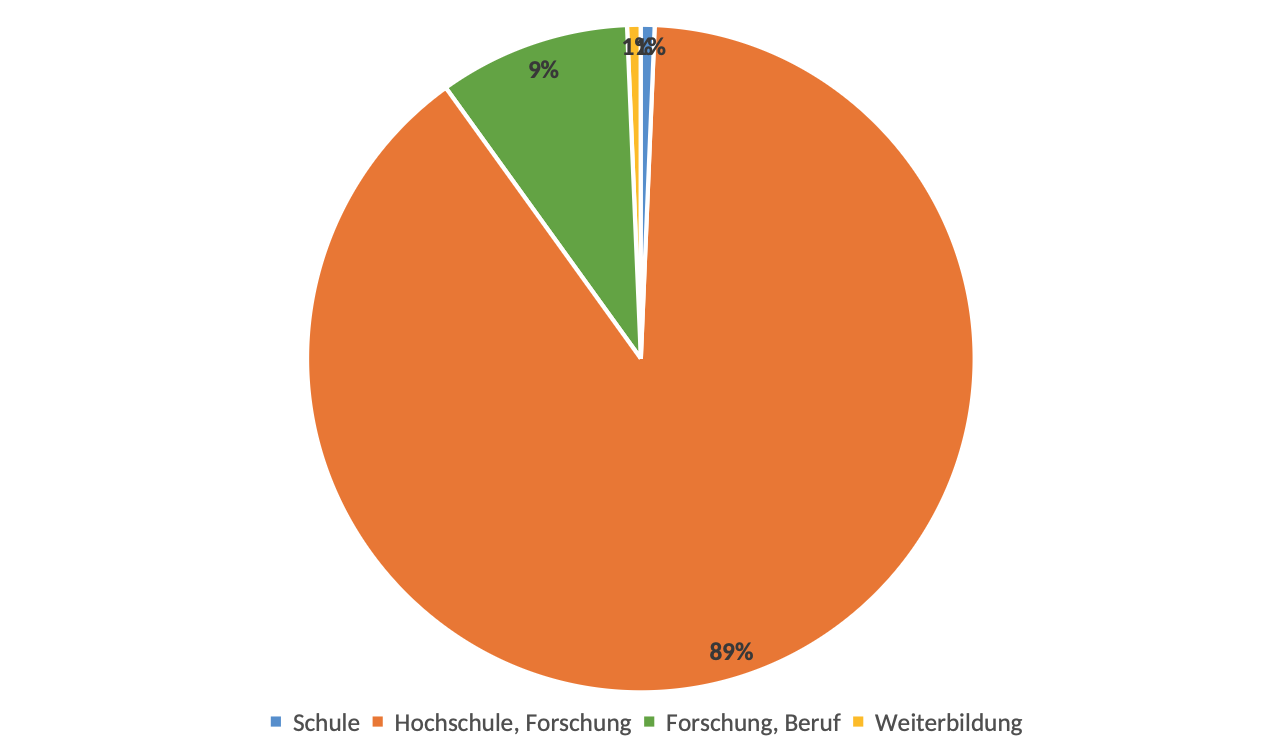
\includegraphics[width=0.90\textwidth]{graphics_lit/9-institution.png}
        \caption{Aufteilung Institutionen}
        \label{fig:9-institution}
    \end{subfigure}
    \hfill
    % 
    % --- rechte Seite: Grafik ---
    \begin{subfigure}[b]{0.48\textwidth}
        \centering
        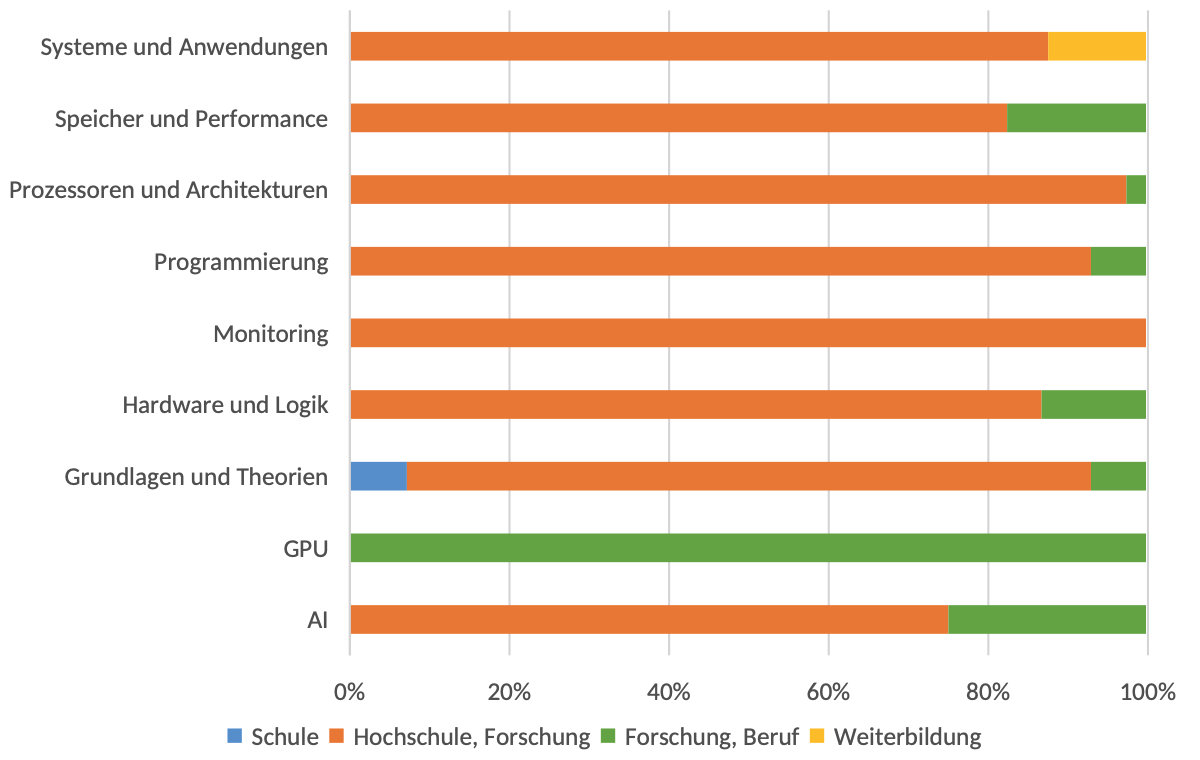
\includegraphics[width=0.90\textwidth]{graphics_lit/10-institution-themen.png}
        \caption{Aufteilung Institutionen nach Themen}
        \label{fig:10-institution-themen}
    \end{subfigure}
    %
    \caption{Analysen zu Institutionen}
    \label{fig:institution-analysen}
\end{figure}

Hinsichtlich des Zugriffs zeigt Abbildung~\ref{fig:11-zugriff} eine detaillierte Aufteilung. Die meisten Simulatoren (ca. 66~\%) sind offline nutzbar, während 11~\% entweder ausschließlich online oder sowohl online als auch offline verfügbar sind. In 19 Publikationen (ca. 13~\%) finden sich keine Angaben zur Art der Nutzung.

\begin{figure}[!htbp]
    \centering
    % --- linke Seite: Grafik ---
    \begin{subfigure}[b]{0.48\textwidth}
        \centering
        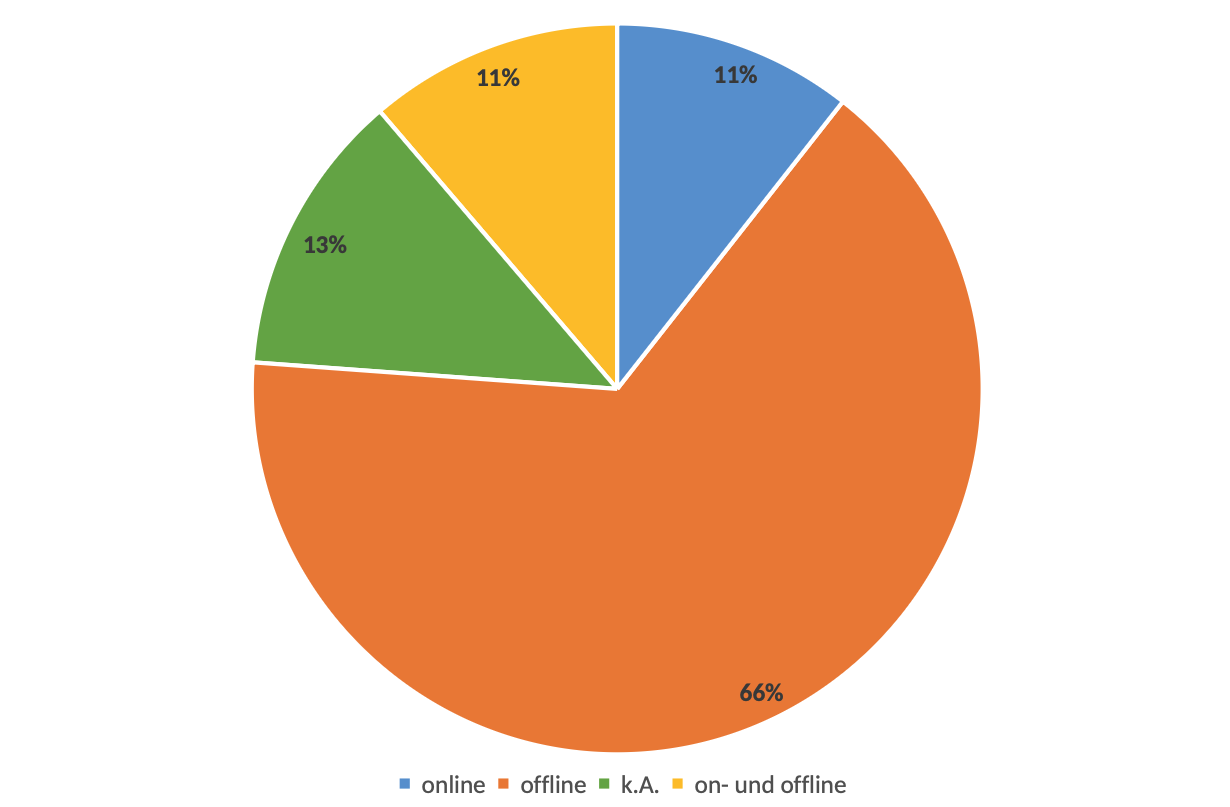
\includegraphics[width=0.90\textwidth]{graphics_lit/11-zugriff.png}
        \caption{Aufteilung Zugriff}
        \label{fig:11-zugriff}
    \end{subfigure}
    \hfill
    % 
    % --- rechte Seite: Grafik ---
    \begin{subfigure}[b]{0.48\textwidth}
        \centering
        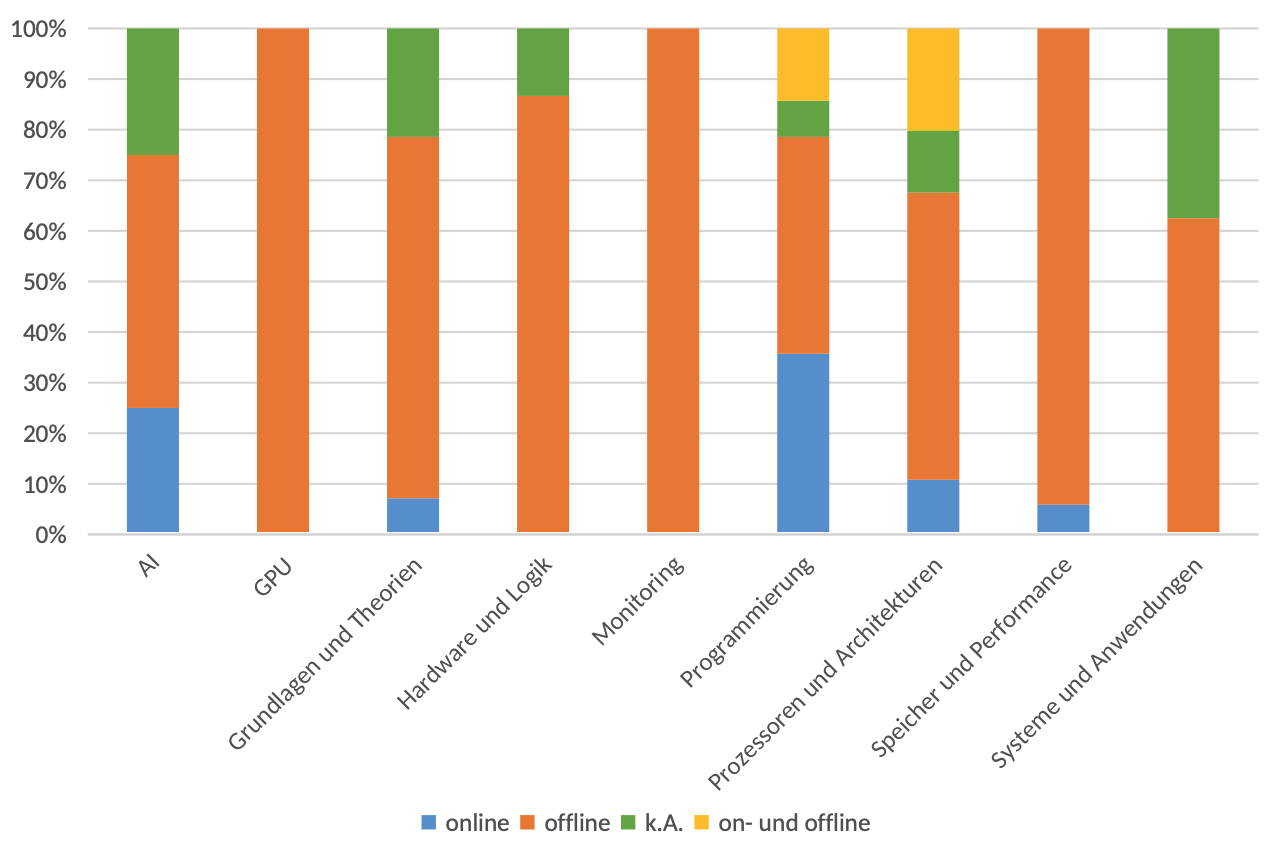
\includegraphics[width=0.90\textwidth]{graphics_lit/13-zugriff-thema.png}
        \caption{Zugriffsart pro Thema}
        \label{fig:13-zugriff-thema}
    \end{subfigure}
    %
    \caption{Analysen zu zum Zugriff}
    \label{fig:zugriff-analysen}
\end{figure}

Die zeitliche Verteilung der verschiedenen Zugriffsarten ist in Abbildung~\ref{fig:12-zugriff-jahr} dargestellt, die entsprechenden Werte sind in Tab.~\ref{tab:zugriff-zeit} aufgeführt.

\begin{figure}[!htbp]
    \centering
    % --- linke Seite: Grafik ---
    \begin{subfigure}[b]{0.48\textwidth}
        \centering
        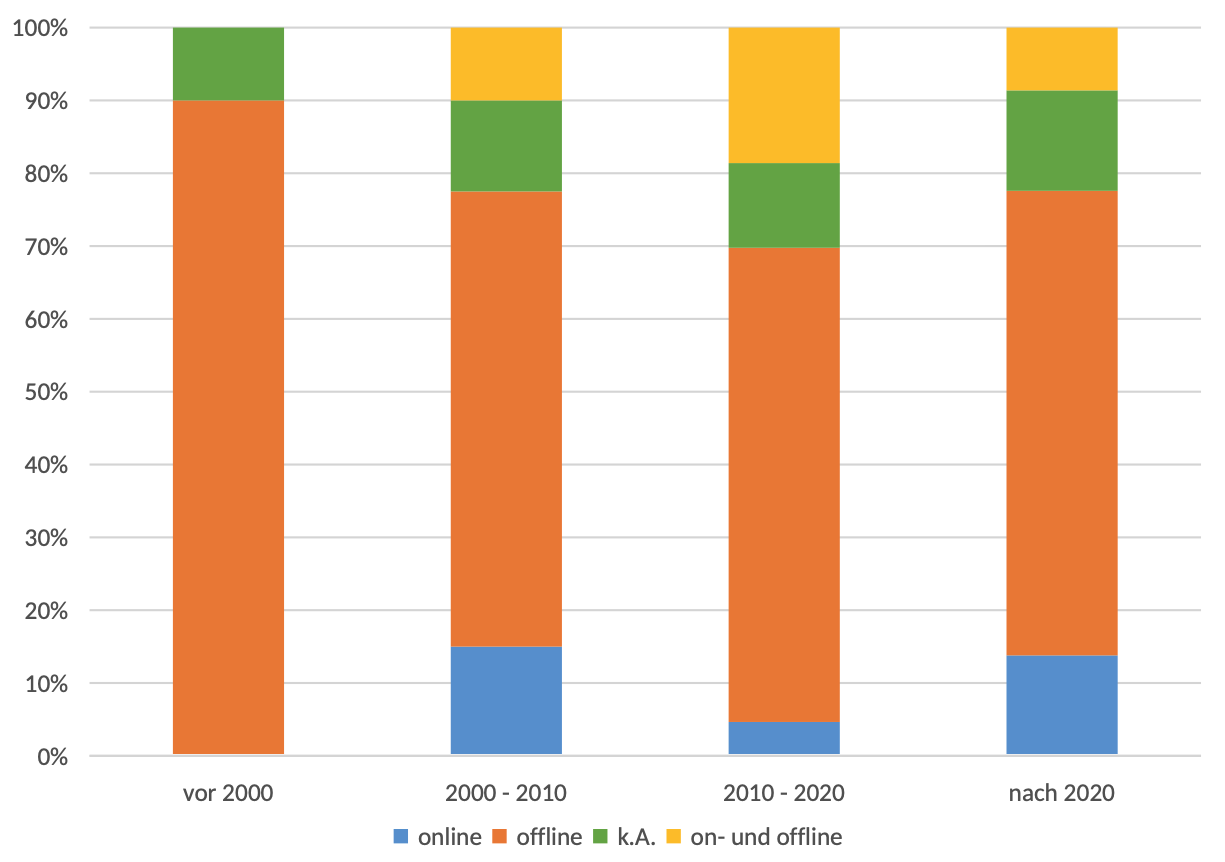
\includegraphics[width=\textwidth]{graphics_lit/12-zugriff-jahr.png}
        \caption{Jährliche Aufteilung Zugriff (grafisch)}
        \label{fig:12-zugriff-jahr}
    \end{subfigure}
    \hfill
    % 
    % --- rechte Seite: Tabelle ---
    \begin{subfigure}[b]{0.48\textwidth}
        \centering
        \tiny
        \begin{tabularx}{\textwidth}{lXXXX}
            \hline
            \textbf{Zeitraum} & \textbf{online} & \textbf{offline} & \textbf{keine Info} & \textbf{on-/offline} \\
            \hline
            vor 2000      & 0  & 9  & 1 & 0 \\
            2000--2010    & 6  & 25 & 5 & 4 \\
            2010--2020    & 2  & 28 & 5 & 8 \\
            nach 2020     & 8  & 37 & 8 & 5 \\
            \hline
        \end{tabularx}
        \caption{Jährliche Aufteilung Zugriff (detailliert)}
        \label{tab:zugriff-zeit}
    \end{subfigure}
    %
    \caption{Darstellung der Zugriffsarten pro Zeitraum}
    \label{fig:zugriff-gesamt}
\end{figure}

Abbildung~\ref{fig:13-zugriff-thema} zeigt die Verteilung der verschiedenen Zugriffsarten in Bezug auf die einzelnen Themenbereiche. Simulatoren, die auf Hardware wie \ac{FPGA}s basieren, werden der Kategorie \enquote{offline} zugeordnet.

Als zusätzliches Kriterium wurde der Preis untersucht, wobei zwischen \enquote{kostenlos} und \enquote{kostenpflichtig} unterschieden wird. Der Anteil der kostenlos verfügbaren didaktischen Simulatoren beträgt 57~\%, während 7~\% kostenpflichtig sind. Für die übrigen Simulatoren liegen keine Angaben zur preislichen Gestaltung vor (vgl. Abbildung~\ref{fig:14-preis2}). 

Darüber hinaus werden die Preiskategorien nach Zeiträumen aufgeschlüsselt, um einen Überblick über mögliche Veränderungen des Verhältnisses von kostenlosen zu kostenpflichtigen Simulatoren zu erhalten (vgl. Abbildung~\ref{fig:15-preis-gesamt}).

\begin{figure}[!htbp]
    \centering
    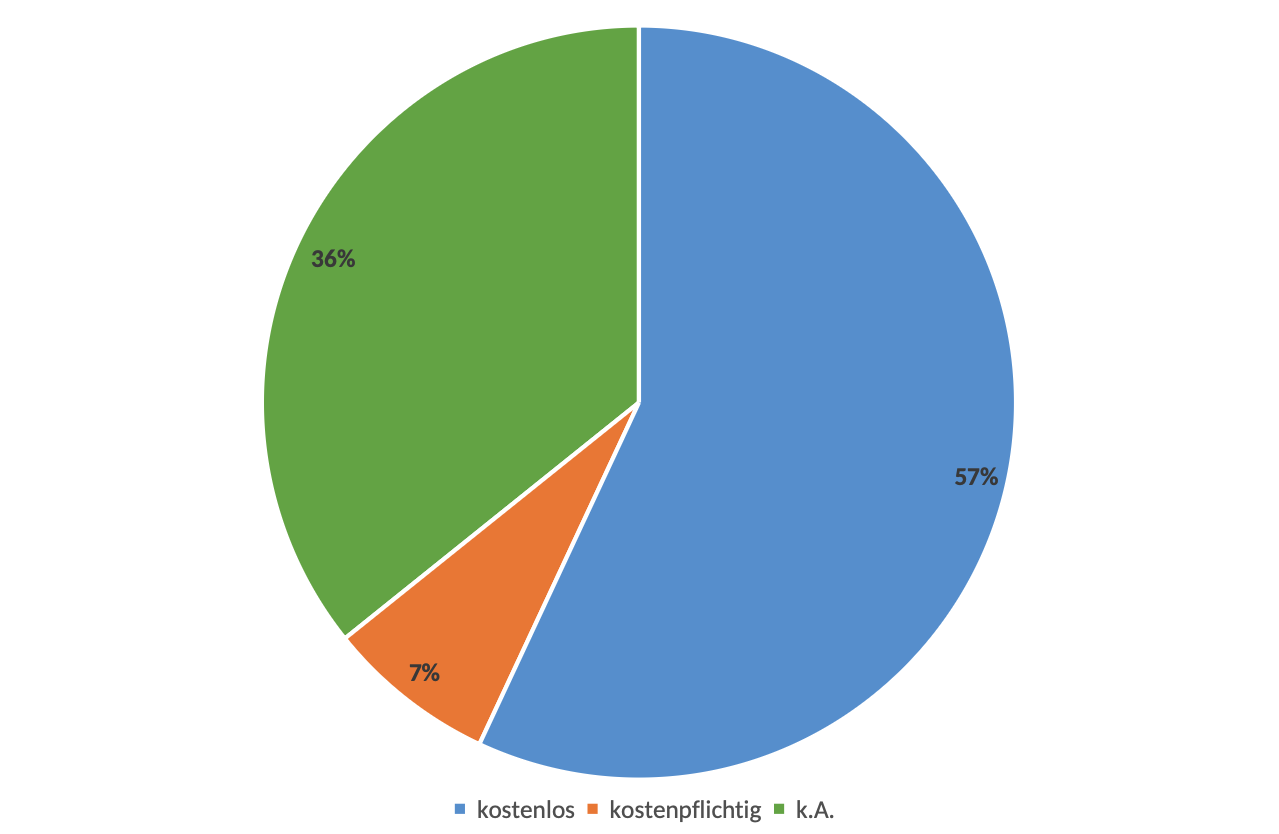
\includegraphics[width=0.9\textwidth]{graphics_lit/14-preis.png}
    \caption{Aufteilung Preis}
    \label{fig:14-preis2}
\end{figure}

\begin{figure}[!htbp]
    \centering
    % --- linke Seite: Grafik ---
    \begin{subfigure}[b]{0.48\textwidth}
        \centering
        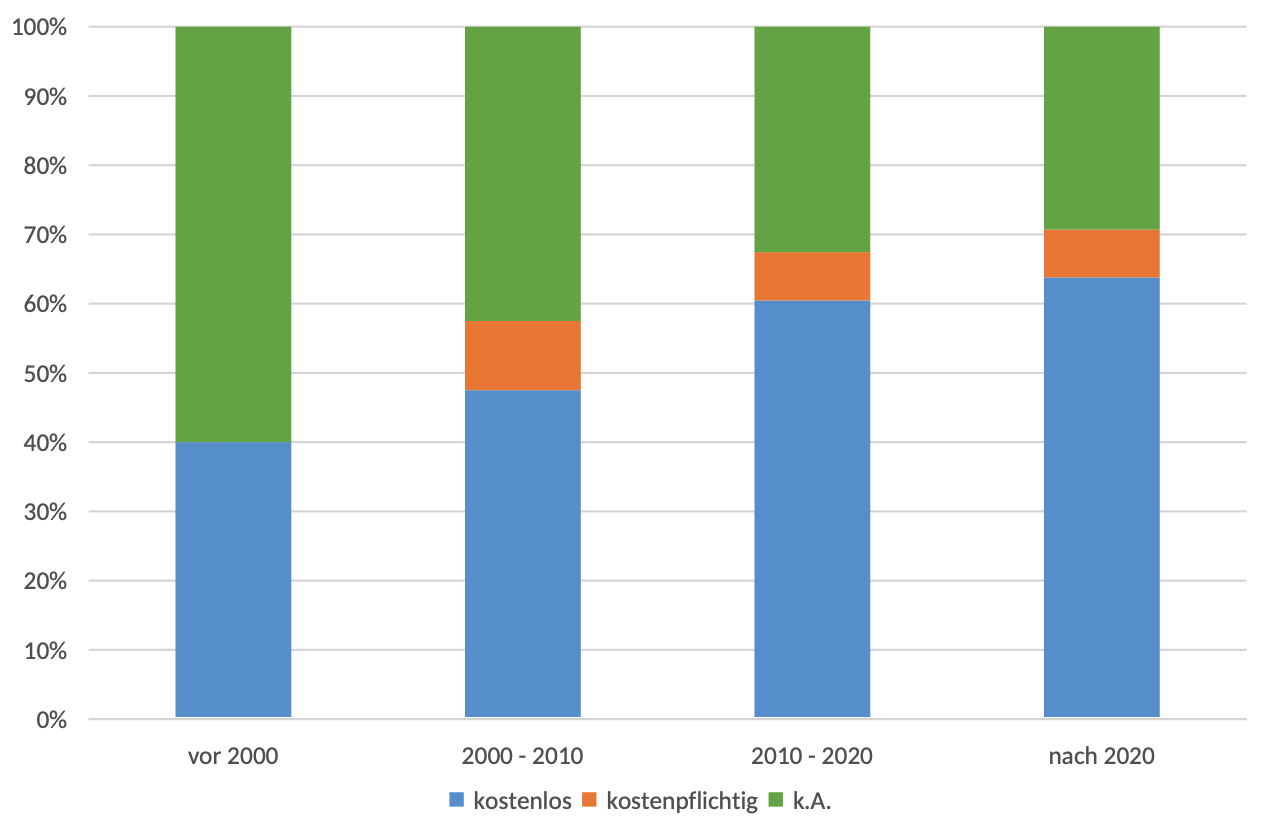
\includegraphics[width=\textwidth]{graphics_lit/15-preis-jahr.png}
        \caption{Aufteilung Preis (grafisch)}
        \label{fig:15-preis-jahr}
    \end{subfigure}
    \hfill
    % --- rechte Seite: Tabelle ---
    \begin{subfigure}[b]{0.48\textwidth}
        \centering
        \tiny
        \begin{tabularx}{\textwidth}{lXXX}
            \hline
            \textbf{Zeitraum} & \textbf{kostenlos} & \textbf{kostenpflichtig} & \textbf{k.A.} \\
            \hline
            vor 2000      & 4  & 0 & 6  \\
            2000--2010    & 19 & 4 & 17 \\
            2010--2020    & 26 & 3 & 14 \\
            nach 2020     & 37 & 4 & 17 \\
            \hline
        \end{tabularx}
        \caption{Aufteilung Preis (detailliert)}
        \label{tab:15-preis-zeit}
    \end{subfigure}
    %
    \caption{Darstellung der Preisgestaltung der Simulatoren über verschiedene Zeiträume}
    \label{fig:15-preis-gesamt}
\end{figure}

In Bezug auf das Kriterium \textit{Dokumentation} gibt Abbildung~\ref{fig:16-dokumentation} genauere Einblicke. In 87~\% der analysierten Publikationen verfügen die verwendeten bzw. beschriebenen Simulatoren über eine Dokumentation, während 5~\% keine Dokumentation erwähnen und in 7~\% der Publikationen hierzu keine Angaben vorliegen.

\begin{figure}[!htbp]
    \centering
    \caption{Aufteilung Dokumentation}
    \label{fig:16-dokumentation}
    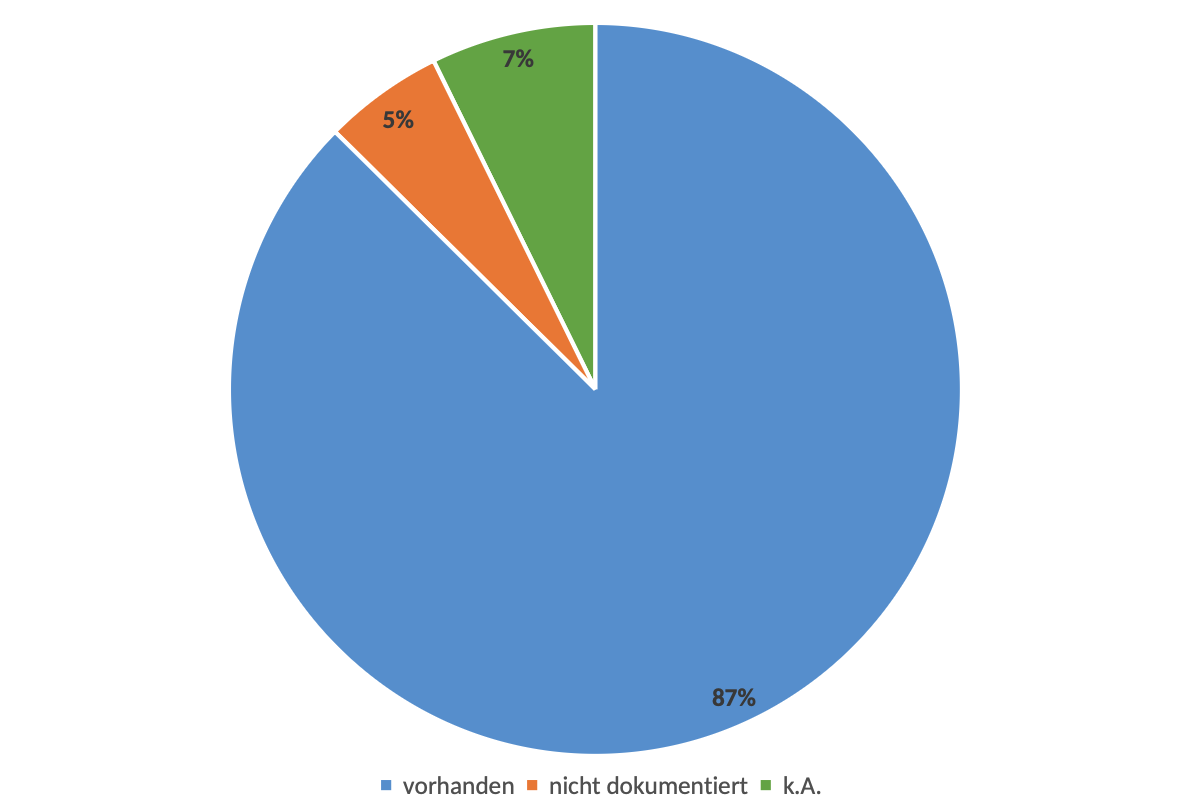
\includegraphics[width=0.90\textwidth]{graphics_lit/16-dokumentation.png}
\end{figure}

Als abschließendes Kriterium wird die Anzahl der Zitationen untersucht. Tabelle~\ref{tab:zitationen} zeigt die am häufigsten zitierten Publikationen pro Thema, da diese für weiterführende oder aufbauende Untersuchungen in den jeweiligen Bereichen als maßgeblich gelten. Die Auswahl der dargestellten Publikationen erfolgte auf Grundlage des Durchschnitts aller Zitationen, der bei etwa 35 liegt. Publikationen mit mehr als 35 Zitationen werden nachfolgend dargestellt.

{
\tiny
\centering
\begin{longtable}{|c|p{6cm}|p{3cm}|c|}
    \caption{Häufig zitierte Publikationen pro Themengebiet\label{tab:zitationen}} \\
    \hline
    \textbf{Zitationen} & \textbf{Titel} & \textbf{Autor(en)} & \textbf{Jahr} \\
    \hline
    \endfirsthead

    \hline
    \textbf{Zitationen} & \textbf{Titel} & \textbf{Autor(en)} & \textbf{Jahr} \\
    \hline
    \endhead

    \hline
    \multicolumn{4}{l}{Fortsetzung auf der nächsten Seite} \\
    \hline
    \endfoot

    \hline
    \endlastfoot

    % --- Inhalte ---
    \multicolumn{4}{c}{\textbf{AI}} \\
    \hline
    211 & Teaching CS50 with AI: Leveraging Generative Artificial Intelligence in Computer Science Education & R. Liu, C. Zenke, C. Liu, A. Holmes, P. Thornton, D. J. Malan & 2024 \\
    \hline
    \multicolumn{4}{c}{\textbf{GPU}} \\
    \hline
    146 & MGPUSim: Enabling Multi-GPU Performance Modeling and Optimization & Y. Sun, T. Baruah, S. A. Mojumber, S. Dong, X. Gong, S. Treadway & 2019 \\
    397 & Accel-Sim: An Extensible Simulation Framework for Validated GPU Modeling & M. Khairy, Z. Shen, T. M. Aamodt, T. G. Rogers & 2020 \\
    \hline
    \multicolumn{4}{c}{\textbf{Grundlagen und Theorien}} \\
    \hline
    117 & Flexible Web-Based Educational System for Teaching Computer Architecture and Organization & J. Djordjevic, B. Nikolic, A. Milenkovic & 2005 \\
    \hline
    \multicolumn{4}{c}{\textbf{Hardware und Logik}} \\
    \hline
    46 & Harnessing FPGAs for Computer Architecture Education & M. Holland, J. Harris, S. Hauck & 2003 \\
    \hline
    \multicolumn{4}{c}{\textbf{Programmierung}} \\
    \hline
    41 & Using Simulators for Teaching Computer Organization and Architecture & P. W. C. Prasad, A. Alsadoon, A. Beg, A. Chan & 2016 \\
    51 & MarieSim: The MARIE Computer Simulator & L. Null, J. Lobur & 2003 \\
    \hline
    \multicolumn{4}{c}{\textbf{Prozessoren und Architekturen}} \\
    \hline
    162 & Control Flow Modeling in Statistical Simulation for Accurate and Efficient Processor Design Studies & L. Eeckhout, R. H. Bell, B. Stougie, K. De Bosschere, L. K. John & 2004 \\
    172 & Applying a Constructivist and Collaborative Methodological Approach in Engineering Education & L. Moreno, C. Gonzalez, I. Castilla, E. Gonzalez, J. Sigue & 2007 \\
    327 & Measuring Experimental Error in Microprocessor Simulation & R. Desikan, D. Burger, S. W. Keckler & 2001 \\
    \hline
    \multicolumn{4}{c}{\textbf{Speicher und Performance}} \\
    \hline
    53 & Cryogenic Computer Architecture Modeling with Memory-Side Case Studies & L. Gyu-Hyeon, M. Dongmoon, B. Ilkwon, K. Jangwoo & 2019 \\
    205 & A Simulation Based Study of TLB Performance & A. Borg, J. B. Chen, N. P. Jouppi & 1992 \\
    \hline
    \multicolumn{4}{c}{\textbf{Systeme und Anwendungen}} \\
    \hline
    139 & Virtual Reality in Computer Science Education: A Systematic Review & J. Priker, A. Dengel, M. Holly, S. Safikani & 2020 \\
    \hline
\end{longtable}
}





\section{Ergebnisse aus Tabelle~\ref{tab:simulatoren}}

test test


\chapter{Diskussion und Best Practices}\label{chap:5-discussion}

% E-Learning
E-Learning ist nicht das gelbe vom Ei\label{elearning}. Niegemann arbeitet in seinem Lehrbuch auf dem Jahr 2009 heraus, dass die Euphorie für E-Learning etwas seit 2002 abzuflachen schien, da viele Erwartungen nicht erfüllt würden.\parencite[S.~14]{niegemann_kompendium_2008}

\begin{itemize}
	\item Kosteneinsparungen könnten häufig nicht erzielt werden, sodass didaktisch wertvolle Lernsoftware mit erhöhten finanziellen Aufwendugen verbunden sei.
	\item Ob Texte und Bilder nun in einer Lernsoftware oder in einem Vorlesungsskript dargestellt werde, weise keinen großen Unterschied auf, da es lediglich Texte und Bilder blieben.
	\item Eine erhöhte Abbrruchrate beim E-Learning sei zu verzeichnen, da die Lernenden das selbstständige Lernen nicht gewohnt seien und keine hinreichende tutorielle Unterstützung erhielten.
	\item Der Zeitaufwand sei beim problembasierten bzw. entdeckenden Lernen in multimedialen Lernumgebungen hoch, sodass auch bei nachgewiesener Effektivität dieser Medien nicht alle Lerninhalte vermittelt werden könnten; die Effektivität des problembasierten Lernens sei zudem keineswegs belegt.
	\item In virtuellen Arbeitsgruppen im Web zeigten sich genau die gleichen Probleme, die von Präsenzarbeitsgruppen bekannt seien.
\end{itemize}

Trotz der oben genannten Schwierigkeiten verdeutlicht Niegemann, dass sich E-Learning als Lehr- und Lernform etabliert habe. Quelle der Probleme sei hier die mangelnde didaktische Konzeption dieser Programme.\parencite[S.~14]{niegemann_kompendium_2008}

% Mobile Learning
Gleichzeitig stellt Mobile Learning neue Anforderungen an Didaktik, Usability und Gestaltung von Lerninhalten, da Bildschirmgröße, Nutzungskontext und Interaktionsmöglichkeiten stärker variieren als bei Desktop-Systemen.

% Microlearning
Es lässt sich festhalten, dass Microlearning eine Reihe zentraler Vorteile bietet: Es fördert zum einen die Behaltensleistung durch die kompakte und wiederholbare Aufbereitung von Lerninhalten. Zum anderen steigert es die Lernendenmotivation und das Engagement, da Inhalte flexibel, kontextbezogen und in kurzen Einheiten vermittelt werden. Darüber hinaus unterstützt Microlearning auch kollaborative Lernprozesse in sozialen oder mobilen Umgebungen. Schließlich zeigen Studien, dass Microlearning die Lernfähigkeit und Leistung der Teilnehmenden insgesamt verbessern kann.\parencite[S.~2]{leong_review_2021}


\section{Trends und Herausforderungen}

\section{Empfehlungen für die Zukunft}

\chapter{Fazit}

Ziel dieser Arbeit war es, den Stand didaktischer Simulatoren für die Lehre der Rechnerarchitektur systematisch zu erfassen, vergleichbar zu machen und daraus Best Practices sowie Entwicklungsperspektiven abzuleiten. Durch die Analyse von 151 Publikationen und 57 veröffentlichten Simulatoren konnten zentrale thematische und didaktische Muster identifiziert werden.

Die Ergebnisse verdeutlichen klare Schwerpunkte: Prozessoren und Architekturen, insbesondere \acs{RISC}, bilden nach wie vor den Kernbereich der didaktischen Simulatoren. Zugleich gewinnen GPU-, KI-bezogene und immersive Ansätze zunehmend an Bedeutung und spiegeln die aktuellen technologischen Entwicklungen der Rechnerarchitektur wider. Damit lassen sich sowohl eine starke Kontinuität klassischer Inhalte als auch erste Verschiebungen hin zu neuen Themenfeldern beobachten.

Didaktisch wirksam sind vor allem reduzierte Darstellungen im Sinne der \acl{CTML}, da sie komplexe Sachverhalte auf wesentliche Kernelemente verdichten. Gamification wird bislang nur vereinzelt integriert, obwohl die Literatur deutliche Potenziale zur Steigerung der Lernmotivation belegt. Häufig genannte Erfolgsfaktoren sind darüber hinaus eine ortsunabhängige Nutzung (online oder hybrid), die Kostenfreiheit, plattformübergreifende Verfügbarkeit sowie eine umfassende und verlässliche Dokumentation. Zusammengenommen führen diese Befunde zu Empfehlungen für die zukünftige Gestaltung, Bereitstellung und didaktische Nutzung von Simulatoren.

Aus der Diskussion ergeben sich zwei zentrale Schlussfolgerungen: Erstens sollten Simulatoren gezielt für kleine, klar strukturierte Lerneinheiten konzipiert werden, die den Lernprozess schrittweise begleiten und bei Bedarf durch spielerische Elemente ergänzt werden können. Zweitens besteht eine deutliche Forschungslücke in Bezug auf belastbare empirische Studien, die den Einsatz dieser Werkzeuge in realen Lehrkontexten untersuchen. Zukünftige Arbeiten sollten daher (1) genauere und weniger subjektive Maße zur Einschätzung der Relevanz nutzen, (2) die Nutzungsdauer und Interaktionsmuster als Indikatoren für Qualität und Motivation erfassen und (3) den schulischen Bildungsbereich stärker berücksichtigen, da Simulatoren bislang vorwiegend in der Hochschullehre verankert sind.

Darauf aufbauend ergibt sich eine Forschungsagenda, die von methodisch fundierten Feldstudien bis hin zur Entwicklung klarer Kategorien reicht, mit denen sich die Unterschiede zwischen \enquote{Gamified Learning} und \enquote{Game-Based Learning} systematisch erfassen lassen. Für die Praxis bedeutet dies, dass Lehrende bereits heute auf eine Reihe Gestaltungsprinzipien zurückgreifen können, während die Forschung in den kommenden Jahren verstärkt Evidenz für Wirksamkeit und Transferfähigkeit liefern sollte. Auf diese Weise trägt die Arbeit sowohl zur theoretischen Fundierung als auch zur praktischen Weiterentwicklung didaktischer Simulatoren im Bereich der Rechnerarchitektur bei.



\cleardoublepage
\clearpage

\listoffigures
\clearpage

\listoftables
\clearpage

\appendix
\csvautotabular[respect all]{tables/Literaturrecherche_clean.csv}


\printbibliography
\MakeBibliography[nosplit]

\end{document}
